\documentclass[tikz,border=5pt]{standalone}
\usepackage{pgfplots}
\pgfplotsset{compat=1.18}

\definecolor{corba}{HTML}{365FB3}
\definecolor{punt}{HTML}{B91C1C}
\definecolor{assimptota}{HTML}{6B7280}

\begin{document}
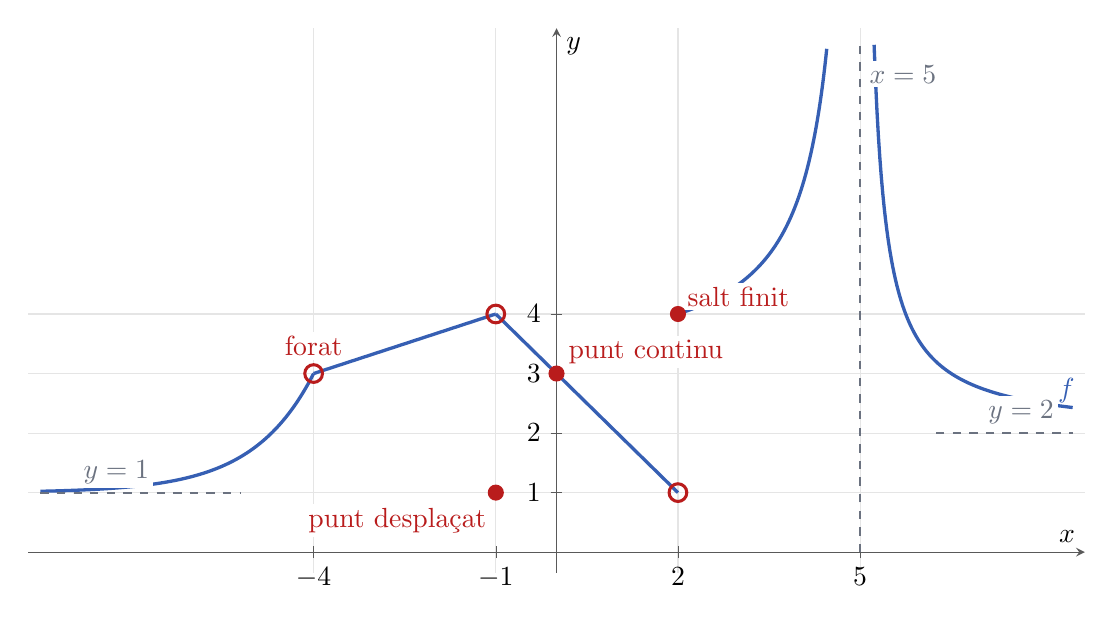
\begin{tikzpicture}
  \begin{axis}[
    width=15cm,
    height=8.5cm,
    axis lines=middle,
    xmin=-8.7,
    xmax=8.7,
    ymin=-0.35,
    ymax=8.8,
    xlabel={$x$},
    ylabel={$y$},
    xtick={-4,-1,0,2,5},
    ytick={1,2,3,4},
    axis line style={black!65},
    tick style={black!65},
    grid=major,
    grid style={black!10},
    clip=false,
  ]
    % Branca esquerra: asímptota horitzontal y=1 quan x tendeix a -infinit.
    \addplot[corba, very thick, domain=-8.5:-4, samples=120]
      {1 + 2*exp(x+4)};

    % Tram entre els dos tipus de discontinuïtat evitable.
    \addplot[corba, very thick, domain=-4:-1, samples=2]
      {3 + (x+4)/3};

    % Tram amb un punt continu a x=0 i límit lateral esquerre 1 a x=2.
    \addplot[corba, very thick, domain=-1:2, samples=2]
      {3-x};

    % Branca que comença després del salt i tendeix a +infinit en x=5.
    \addplot[corba, very thick, domain=2:4.45, samples=140]
      {3 + 3/(5-x)};

    % Branca dreta: asímptota vertical x=5 i horitzontal y=2.
    \addplot[corba, very thick, domain=5.23:8.5, samples=140]
      {2 + 1.5/(x-5)};

    % Asímptotes.
    \addplot[assimptota, dashed, thick, domain=-8.5:-5.2] {1};
    \node[assimptota, fill=white, inner sep=1.5pt] at (axis cs:-7.25,1.35) {$y=1$};
    \addplot[assimptota, dashed, thick, domain=6.25:8.5] {2};
    \node[assimptota, fill=white, inner sep=1.5pt] at (axis cs:7.65,2.35) {$y=2$};
    \draw[assimptota, dashed, thick]
      (axis cs:5,0) -- (axis cs:5,8.55);
    \node[assimptota, fill=white, inner sep=1.5pt, anchor=south west]
      at (axis cs:5.08,7.8) {$x=5$};

    % Punts oberts: forat, punt desplaçat i extrem esquerre del salt.
    \addplot[
      only marks,
      mark=o,
      mark size=3.2pt,
      mark options={draw=punt, fill=white, line width=1.1pt}
    ] coordinates {(-4,3) (-1,4) (2,1)};

    % Punts definits: valor desplaçat, punt continu i extrem dret del salt.
    \addplot[
      only marks,
      mark=*,
      mark size=2.7pt,
      mark options={draw=punt, fill=punt}
    ] coordinates {(-1,1) (0,3) (2,4)};

    % Etiquetes que ajuden a identificar cada fenomen.
    \node[punt, fill=white, inner sep=1.5pt, anchor=south]
      at (axis cs:-4,3.22) {forat};
    \node[punt, fill=white, inner sep=1.5pt, anchor=north east]
      at (axis cs:-1.08,0.82) {punt desplaçat};
    \node[punt, fill=white, inner sep=1.5pt, anchor=south west]
      at (axis cs:0.12,3.08) {punt continu};
    \node[punt, fill=white, inner sep=1.5pt, anchor=south west]
      at (axis cs:2.08,4.05) {salt finit};
    \node[corba, anchor=west] at (axis cs:8.1,2.72) {$f$};
  \end{axis}
\end{tikzpicture}
\end{document}
